\documentclass[a4paper,14pt,href]{article}

% Используем нестандартный размер шрифта
\usepackage{extsizes}

% Делаем отступ для первого параграфа
\usepackage{indentfirst}

% Для поддержки поиска по pdf документу
\usepackage{cmap}

% Поддержка кириллицы
\usepackage[T2A]{fontenc}
\usepackage[utf8]{inputenc}
\usepackage[english,russian]{babel}

% Поддержка списков
\usepackage{enumerate}

% Заменяем библиографию с квадратных скобок на точку
\makeatletter
\renewcommand{\@biblabel}[1]{#1.}
\makeatother

% Графический пакет
\usepackage{graphicx}
\usepackage{epstopdf}
\usepackage{tikz}

% Математические шрифты AMS
\usepackage{amstext, amssymb, amsmath}

% В заголовках появляется точка, но при ссылке на них ее нет
\usepackage{misccorr}

% Поддержка гиперссылок
\usepackage{url}

% Задаем полуторный межстрочный интервал
\linespread{1.3}

% Задаем глубину оглавления
\setcounter{tocdepth}{2}

% Путь к изображениям, по умолчанию
\graphicspath{{images/}}

% Задаем отступ абзаца
\setlength{\parindent}{1.25cm}

\renewcommand{\labelenumi}{\arabic{enumi}.}% Меняем везде перечисления на цифра.цифра

% Меняем поля страницы
\usepackage{geometry}
\geometry{left=2.5cm}   % левое поле
\geometry{right=2.5cm}  % правое поле
\geometry{top=2.5cm}    % верхнее поле
\geometry{bottom=2.5cm} % нижнее поле


% Листинг
\usepackage{listings}
\usepackage{color}
\usepackage{xcolor}

\usepackage{caption}
\DeclareCaptionFont{white}{\color{white}}
\DeclareCaptionFormat{listing}{\colorbox{gray}{\parbox{\textwidth}{#1#2#3}}}
\captionsetup[lstlisting]{format=listing,labelfont=white,textfont=white}

\renewcommand{\lstlistingname}{Листинг}

\lstset{
  caption=Листинг,
  basicstyle=\footnotesize\ttfamily,
  numbers=left,
  numberstyle=\color{gray}\tiny,
  numbersep=5pt,
  tabsize=2,
  extendedchars=false,
  xleftmargin=17pt,
  framexleftmargin=17pt,
  framexrightmargin=5pt,
  framexbottommargin=4pt,
  showstringspaces=false,
  keepspaces = true}



\begin{document}


%%%
% Титульный лист
%%%
\thispagestyle{empty}
\begin{center}
Федеральное государственное автономное образовательное учреждение \\
высшего профессионального образования \\
\textsc{<<Южный Федеральный Университет>>}\\[1.0cm]

Факультет математики, механики и компьютерных наук\\[1.0cm]

Направление подготовки 010400 \\
<<Прикладная математика и информатика>>\\[3cm]

А. А. Тактаров \\[1.0cm]
\textsc{Реактивный фреймворк для организациии мультиагентных распределенных вычислений}\\[1.0cm]

\textit{Магистерская диссертация}\\[2.0cm]

\begin{flushright}
    Научный руководитель: \\
    старший преподаватель \\
    В. Н. Брагилевский \\[1.0cm]

    Рецензент: \\
    доцент, к. ф.-м. н.\\
    С. А. Гуда
\end{flushright}

\vfill

  Ростов-на-Дону\\
  2014
\end{center}

\newpage
\tableofcontents

\newpage
\section*{Введение}
\addcontentsline{toc}{section}{Введение}

Стремительный рост возможностей технологий беспроводной передачи данных, а также широкое распространение мобильных и
встраиваемых устройств способоствовали появлению концепции так называемого <<Интернета вещей>>
(англ. \textit{<<Internet of Things>>})\cite{IoTWired}, которая заключается в объединении всех окружающих людей вещей в
огромную вычислительную сеть. Участниками (\textit{агентами}) такой сети являются устройства, которые способны собирать
информацию о физической среде, обрабатывать ее и реагировать на изменение состояния других агентов и всей системы в целом.
Стабильное функционирование такой сети позволит с огромной скоростью внедрять и использовать такие технологии, как
<<умные>> датчики\cite{NestThermostat}, носимые устройства (англ. \textit{wearable devices}), а также системы
автоматизированного управления домом. Кроме того, становление <<Интернета вещей>> влечет за собой появление
принципиально новых потоков информации, тщательный анализ которых позволит улучшать существующие системы
здравоохранения, безопасности и контролировать состояние окружающей среды.

Однако, создание подобного рода сети невозможно без наличия функционирующей инфраструктуры, которая бы позволила быстро
и эффективно интегрировать новые компоненты. Исходя из распределенной природы описываемой сети, сформулируем необходимые
для этого требования:

\begin{enumerate}
  \item Соблюдение принципа системности при разработке\cite{SystemPrinciple}. Продукт должен быть представлен в виде
  целой системы компонентов, каждый из которых обладает определенной функцией. Такие компоненты автоматически становятся
  автономными участниками сети.

  \item Однородность среды. Компоненты сети должны иметь возможность взаимодействовать между собой, используя
  стандартизированные протоколы и схемы. Задачи идентификации, обеспечения целостности, конфиденциальности передаваемых
  данных должны по возможности быть решены этими протоколами.

  \item Открытость используемых технологий. Применение как программных, так и аппаратных решений, которые имеют
  открытую документацию, лояльные  условия использования и одновременно поддерживаются разными разработчиками
  (обычно целым сообществом), позволяет в определенных случаях решить проблему интеграции компонентов и сократить разрыв
  между разработкой и запуском в производство. Кроме того, открытые платформы предоставляют широкие возможности для
  начинающих команд разработчиков, что является благоприятным для формирования рынка.
\end{enumerate}

В данной работе описан процесс реализации и интеграции муль\-тиагентной системы на примере задачи распределенной
печати фотографий. В рамках разработанной системы устройство, печатающее фотографию, рассматривается как автономный
агент, который обладает состоянием и способен принимать и исполнять задания. Принципы, сформулированные выше, были
использованы в качестве основополагающих на этапах проектирования и разработки данного продукта.

\newpage
\section*{Постановка задачи}
\addcontentsline{toc}{section}{Постановка задачи}
Целью работы является разработка и развертывание системы, позволяющей организовать моментальную печать фотографий
пользователей социальной сети Instagram, распределяя задания печати среди подключенных к системе агентов ---
\textit{печатных станций}, в состав которых входит печатное устройство --- принтер.

\begin{figure}[htbp]
\begin{center}
  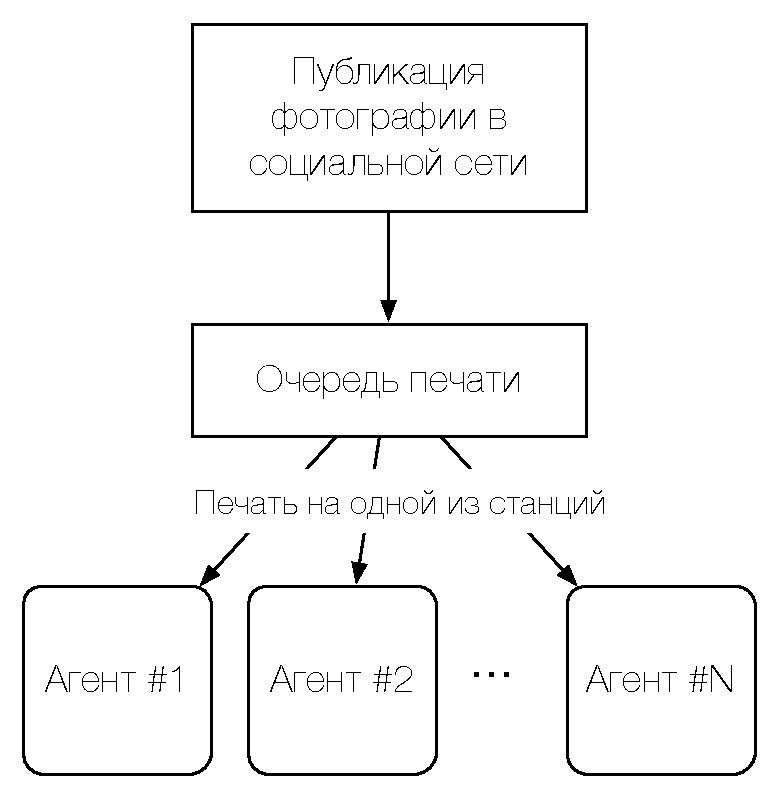
\includegraphics[scale=0.7]{print_schema.pdf}
    \caption{Схема исполнения заданий печати}
    \label{fig:PrintSchema}
\end{center}
\end{figure}

Фотографии, которые публикуются пользователями социальной сети и удовлетворяют определенным условиям поиска
(содержат заранее известную метку --- \textit{хештег}), должны автоматически поступать в очередь печати системы.
Далее, исходная фотография, прошедшая определенную пост-обработку, печатается на одном из принтеров, входящими в
состав печатных станций (рис. \ref{fig:PrintSchema}). Информация о напечатанной фотографии сохраняется в системе для
отчетности. Функционирование такой системы позволяет организовать массовую печать фотографий во время проведения
мероприятий или для огранизации отложенной печати.

Сформулируем основные требования, предъявляемые к системе:
\begin{enumerate}
  \item Печатные станции могут быть физически отделены друг от друга, кроме того они могут находиться в разных
  сегментах сети. Необходим способ организации канала связи между агентами и контроль жизнеспособности этого канала.

  \item Необходим интерфейс управления печатными станциями и заданиями печати.

  \item Система должна иметь минимальный отклик и максимально быстро реагировать на изменение состояния компонентов.
  Изменение статуса задания печати (печать может завершиться успешно, а может закончиться неудачей в результате
  обрыва соединения) должно моментально отражаться в интерфейсе управления заданиями.
\end{enumerate}

Выделим последовательные этапы решения поставленной задачи:
\begin{enumerate}
  \item Проектирование архитектуры системы: разбиение системы на компоненты, выбор используемых при реализации
  каждого компонента технологий, построение схемы взаимодействия.

  \item Реализация компонентов системы, покрытие отдельных частей функциональными тестами.

  \item Решение задач интеграции и развертывании системы, настройка аппаратных средств.

  \item Опытное тестирование работы продукта.
\end{enumerate}

\newpage
\section{Архитектура системы}
В состав разработанного продукта входят три основных компонента: центральный сервер, агент печатной станции и
веб-приложение, предоставляющее интерфейс пользователя (рис. \ref{fig:Architecture}).

\begin{figure}[htbp]
\begin{center}
  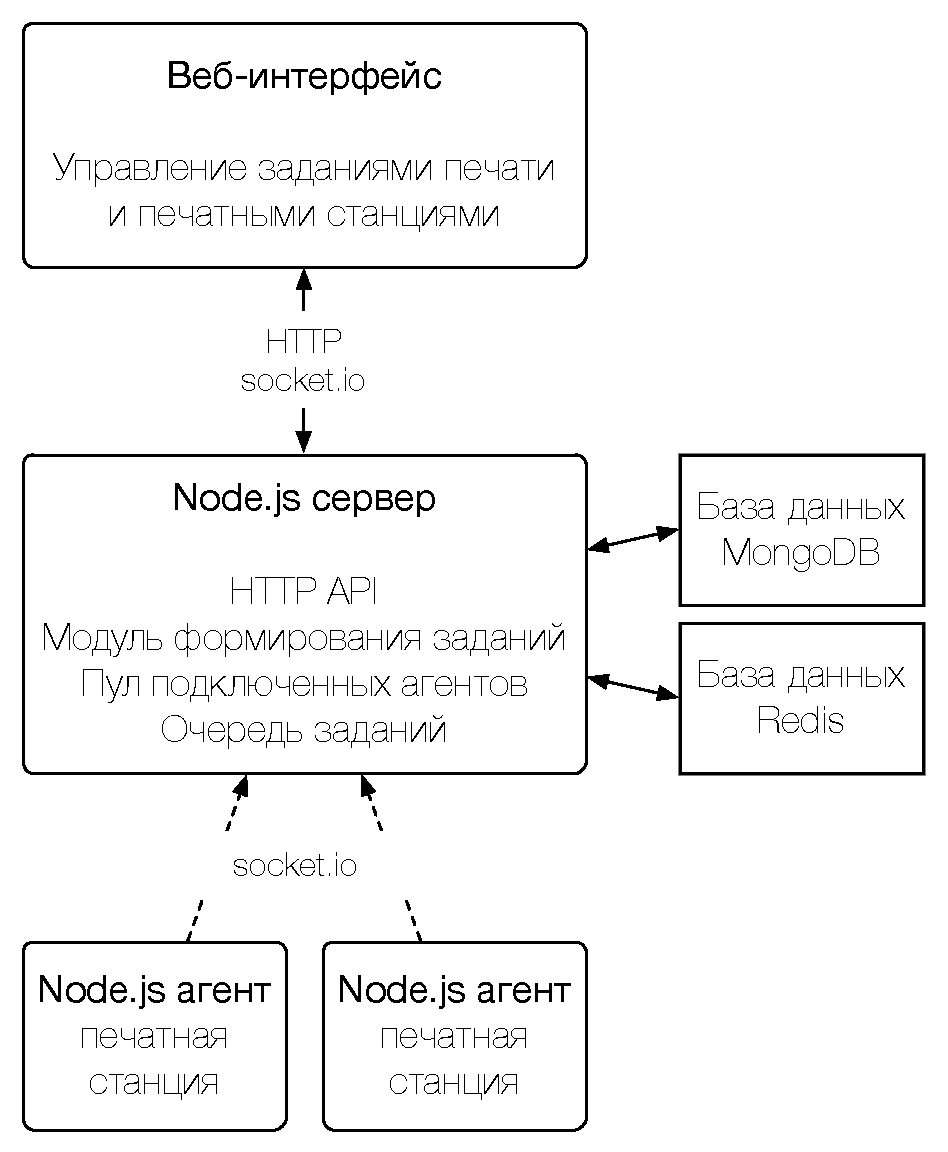
\includegraphics[scale=0.7]{architecture.pdf}
    \caption{Архитектура системы}
    \label{fig:Architecture}
\end{center}
\end{figure}

Для хранения данных используются базы данных MongoDB и Redis, обращение к которым происходит через центральный сервер.
База данных MongoDB содержит информацию о зарегистрированных печатных станциях, администраторах системы, а также хранит
историю всех завершенных заданий печати. Средствами MongoDB реализована возможность гибкого поиска и
фильтрации данных\cite{MongoDBBook}.

База данных Redis, являющаяся быстрым хранилищем типа <<ключ-значение>>, используется для организации очереди
заданий печати. Кроме того, благодаря возможности хранения данных в оперативной памяти данная база данных выступает в
роли хранилища сессий центрального веб-сервера.

\subsection{Центральный сервер}
Ядром системы является центральный сервер, функциями которого являются:

\begin{enumerate}
  \item Управление очередью печати. Модуль формирования заданий используется для поиска в социальной сети новых
  отмеченных для печати фотографий, которые помещаются в очередь печати. Распечатанные фотографий извлекаются из
  очереди, а ненапечатанные дополняются сообщением об ошибке для отчетности.

  \item Взаимодействие с подключенными по каналу связи агентами. Контроль качества канала связи и авторизация
  печатных станций.

  \item Предоставление прикладного программного интерфейса (API) на основе протокола HTTP.
\end{enumerate}

Данный компонент разработан на языке программирования \linebreak CoffeeScript\cite{LittleCoffeeScript} и работает
на основе асинхронного серверного фреймворка Node.js. Решение по использованию данного инструментария было принято,
исходя из следующего:

\begin{enumerate}
  \item Платформа Node.js предоставляет широкие возможности по использованию низкоуровневых средств (работа с
  процессами, сокетами, бинарными данными и потоками ввода-вывода), предоставляя для этого удобный интерфейс на
  языке программирования JavaScript. Кроме того, все операции ввода вывода в Node.js являются асинхронными
  (т.е. не блокируют исполнение программы), а контроль завершения происходит с помощью функций обратного вызова
  и событий. Обработка завершения асинхронных действий реализована в так называемой \textit{очереди обработки событий}
  (англ. \textit{event loop})\cite{UnderstandingEvenLoop}, работающей на основе паттерна Проактор\cite{BoostProactor}.

  \item Node.js позволяет разработчику использовать сторонние модули благодаря мощному пакетному менеджеру NPM.
  Простота публикации модулей и открытое сообщество разработчиков по всему миру способствовали развитию огромной
  инфраструктуры пакетов\cite{NPMGrowth}. Таким образом, проектирование приложений заключается в разбиении на
  мелкие подзадачи, которые решаются с использованием готовых пакетов, что позволяет оптимизировать процесс разработки.

  \item Благодаря тому, что JavaScript является интерпретируемым языком, программы, написанные с использованием
  Node.js, являются кроссплатформенными. Существует поддержка операционных систем, совместимых с ARM-процессорами,
  что делает возможным запуск кода даже на встраиваемых устройствах.

  \item Язык программирования CoffeeScript является компилируемым в \newline JavaScript языком, расширяющим
  возможности последнего за счет полноценной поддержки объектно-ориентированной парадигмы и добавления
  <<синтаксического сахара>>. Синтаксические особенности языка делают возможным реализацию сложных паттернов
  проектирования, что является важным при разработке больших приложений\cite{CoffeeScriptCookbook}.
\end{enumerate}

\subsection{Агент печатной станции}
В представленной системе компонентом, который исполняет задания печати, является агент печатной станции, подключенный к
центральному серверу. В задачи данного модуля входит:

\begin{enumerate}
  \item Принятие заданий печати от центрального сервера, представленных в виде изображения и метаинформации, в которую
  входят параметры печати и другие вспомогательные данные.

  \item Работа с локальной очередью печати подключенного принтера. Постановка на печать полученного изображения.

  \item Отправка отчета о статусе завершенного задания.
\end{enumerate}

Компонент разработан на языке программирования CoffeeScript и работает под управлением фреймворка Node.js. В отличие в
центрального сервера, который функционирует в режиме демона, подразумевается, что агент может быть запущен по требованию.
Более того, одновременно могут быть доступны несколько печатных станций, разнесенных физически и представленных в виде
отдельных экземпляров данного компонента.

\subsection{Организация канала связи между сервером и агентом}
При разработке мультиагентных систем особенно остро встает проблема организации канала связи, который обеспечивает
взаимодействие агентов с сервером, распределяющим задания. При проектировании таких систем становится очевидным, что
невозможно решить данную проблему, используя только возможности протокола TCP. Во-первых, следует учитывать, что
выход в сеть чаще всего всего происходит посредством NAT или межсетевого экрана, что органичивает возможность
подключения (в таких условиях необходимо выделять центральный узел, чаще всего расположенный на выделенном сервере).
Во-вторых, должен быть способ поддержания длительных сессий между участниками (например, опция keepalive\cite{Keepalive}
протокола TCP не реализована в старых версиях ядра Linux). Наконец, традиционная схема передачи данных не является
удобной при реализации реактивных систем, взаимодействие компонентов в которой обычно организовано в виде двунаправленной
передачи сообщений.

В для огранизации канала связи между сервером и печатной станцией в описываемой системе выбор был сделан в пользу
свободно распространяемой библиотеки socket.io\cite{SocketIO}. Данная библиотека предоставляет следующие возможности:

\begin{enumerate}
  \item Организация дуплексного канала связи, который абстрагирован от среды запуска и транспорта. Возможно использование
  socket.io как в серверных и клиентских приложениях (написанных на Node.js), так и в веб-браузере. Для передачи данных
  могут использоваться технологии WebSockets или JSON Polling (периодический опрос сервера о наличии новых сообщений);
  переключение между этими транспортами является прозрачным.

  \item Автоматический контроль жизнеспособности канала. Это реализовано при помощи отправки серии служебных сообщений
  (heartbeats) от клиента к серверу и наоборот. В случае обрыва соединения происходит попытка повторного подключения,
  причем существует стратегия экспоненциального увеличения интервала между неудачными попытками. Такое поведение доступно
  по-умолчанию, и чаще всего процесс восстановления соединения скрыт от программиста.
\end{enumerate}

Узлы, использующие socket.io, обмениваются друг с другом сообщениями, которые сериализуются для отправки выбранным
транспортом. Сообщение можно представить в виде кортежа $(T, a_1, a_2, ..., a_N)$, где $T$ --- текстовый идентификатор
типа сообщения, $a_1, a_2, ..., a_N $ --- сериализованные параметры сообщения.

Библиотека socket.io предоставляет также возможность реализации удаленного вызова процедур (англ. RPC --- Remote
Procedure Call) благодаря механизму подтверждений (англ. \textit{acknowledgement}). Использование удаленного вызова
процедур на примере функции возведения в квадрат представлено в листинге \ref{lst:rpc}. Вызов удаленной функции происходит
как отправка сообщения, последним параметром которого является функция обратного вызова, которая будет исполнена, как только
удаленная сторона отправит ответ. Реализация удаленной функции также содержит параметр-функцию, которую необходимо вызвать
для возврата значения. Заметим, что этот параметр не является исходной функцией, которая была передана при отправке
сообщения. Ее вызов приводит к отправке подтверждающего сообщения, содержащего результат.


\begin{lstlisting}[caption=Удаленный вызов процедур в socket.io, label=lst:rpc]
  # RPC функция возведения числа в квадрат
  socket.on "square", (n, callback) ->
    # Вызов переданной функции выглядит как вызов
    # обычной функции
    callback n * n


  # Вызов RPC функции на клиенте выглядит как отправка сообщения.
  # Первый аргумент: тип сообщения
  # Второй аргумент: параметр сообщения
  # Третий аргумент это функция реакции на acknowledgement
  socket.emit "square", 10, (result) ->
    # Полученный результат: 100
    console.log result
\end{lstlisting}



\newpage
\addcontentsline{toc}{section}{Список литературы}

\bibliographystyle{unsrt}
\bibliography{bibliography/sources}

\end{document}
